% !TeX root = ../thuthesis-example.tex

\chapter{\MakeUppercase{NUIX-Studio Development kit}}

NUIX-Studio Development Kit helps researchers to fast prototype AIoT projects. This chapter briefly introduces each of its components, which are listed below:
\begin{enumerate}
    \item Things designer;
    \item Complex computations API;
    \item API and tools for IoT data visualization and analysis;
    \item API for creating Widgets.
\end{enumerate}

\section{Things Designer}

By using a block structure to represent devices, researchers can modify various parameters of existing devices by changing specific blocks and can create new devices by combining the blocks. This action is possible in a tool called Things designer. This tool is described in detail below.

The Semantic model is visualized inside the Web interface. Researchers can assign Widgets for each of the Items and group the Items together. After the setup is completed, researchers can further develop new devices inside the NUIX-Studio App. Next, they can create new Widgets in Virtual reality and connect them to the existing Items. The position for each of the Widgets is added to the Semantic model as an Item. Having set the Widget's position and other parameters, the user can exit the application on a device and then continue research using a different device or analyze the Item data stored on the server. 

There is a variety of different Widgets available for users. For example, a door open/close sensor with a light indicator can be combined of a Contact sensor Widget and Light Switch Widget (Figure~\ref{fig:PersistenceExample-figure}). Even though the Widgets are created virtually, they get added to the openHAB database. As already mentioned, each Widget is associated with an Item, and the Items together compose a Thing. Thus, a Thing is created, consisting of two Items: a Contact sensor and a light Switch indicator. Further, developers can link the corresponding Channels to each of the Items. For example, researchers can add a Binding for a real-world light bulb, and a Binding for a real-world sensor for opening and closing doors, discover the devices automatically and add them to the model. Next, in the device editing window, bind the Contact sensor and Light Switch sensor to the newly created Items. Thus, the light bulb will light up both in the real and virtual worlds when at least one of the doors is open. The developer can also set the initial state for the open door, solving the problem of synchronizing the door position in the real and virtual worlds. 

\begin{figure}
  \centering
  \subcaptionbox{Opened door.\label{fig:dooropen}}
    {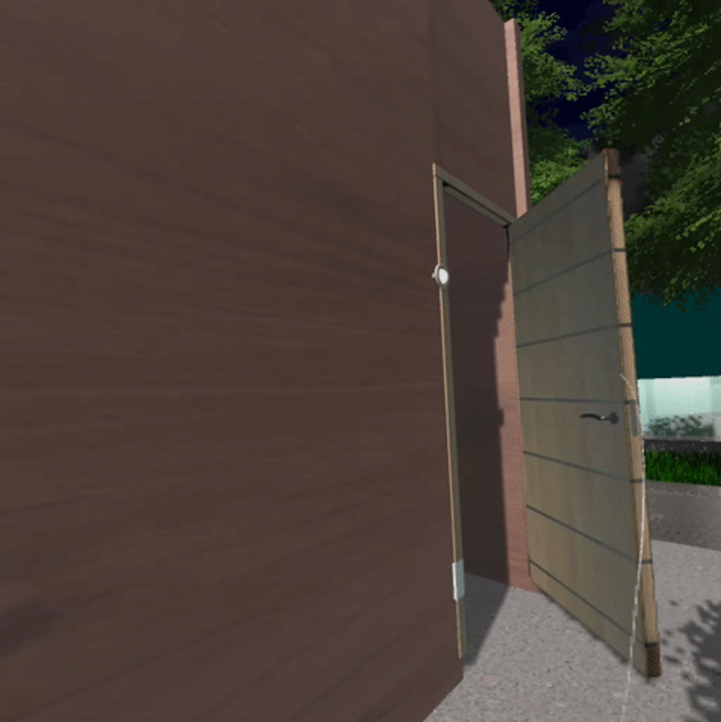
\includegraphics[width=0.45\linewidth]{figures/DoorOpen.png}}
  \subcaptionbox{Closed door.\label{fig:doorclose}}
    {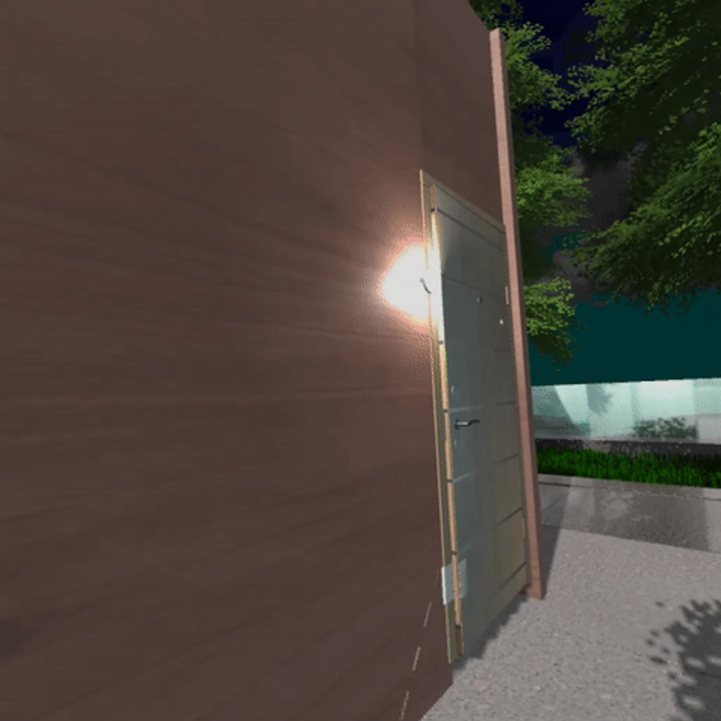
\includegraphics[width=0.45\linewidth]{figures/DoorClose.png}}
  \caption{Door open/close sensor with a light indicator.}
  \label{fig:doorsensor}
\end{figure}

As it was noted, the basic blocks of which the example device consisted are a contact sensor and a switch. As shown in the previous chapter, the platform supports almost all possible Item types presented on the openHAB server. For each item type, there is a corresponding basic Widget. There are 11 basic widgets in total (for example, Dimmer Widget (Figure~\ref{fig:DimmerWidgets-figure}) and Color Picker Widget (Figure~\ref{fig:ColorPickerWidget-figure}) are automatically created for Dimmer and Color Items, respectively). 

\begin{figure}
  \centering
  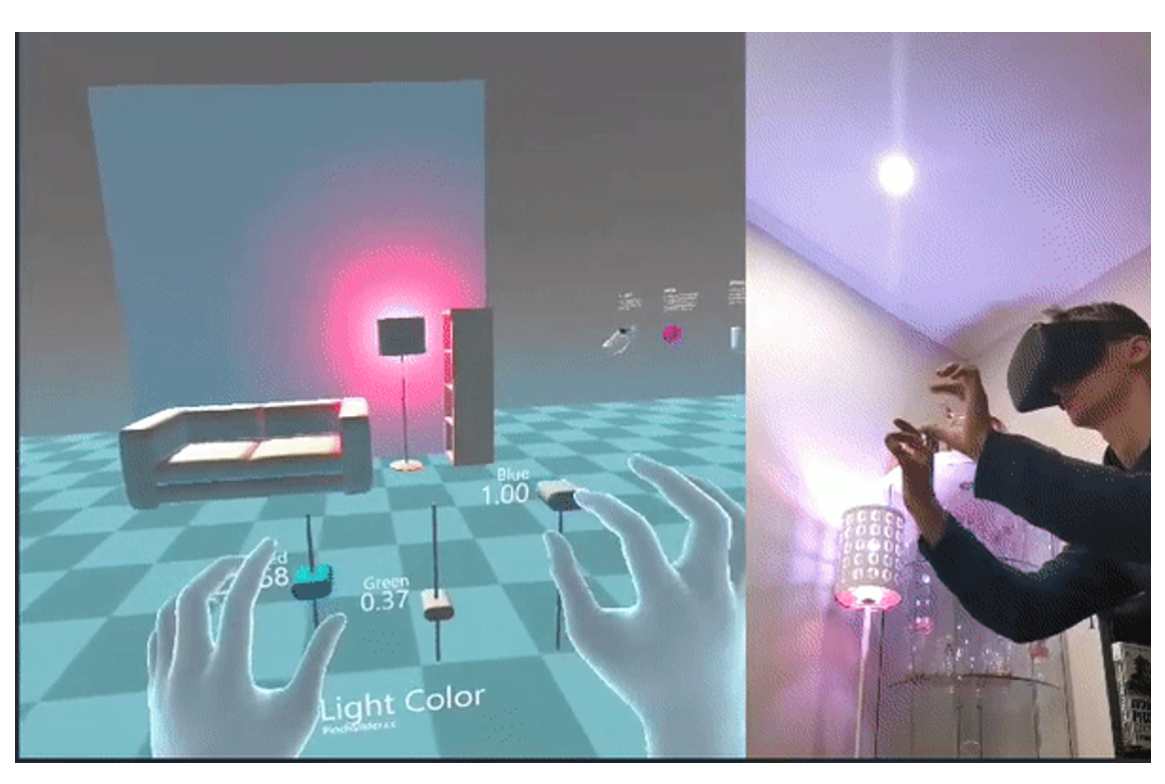
\includegraphics[width=0.9\linewidth]{figures/DimmerWidgets.png}
  \caption{Dimmer Widgets being used to control Red, Green and Blue components of the light.}
  \label{fig:DimmerWidgets-figure}
\end{figure}

\begin{figure}
  \centering
  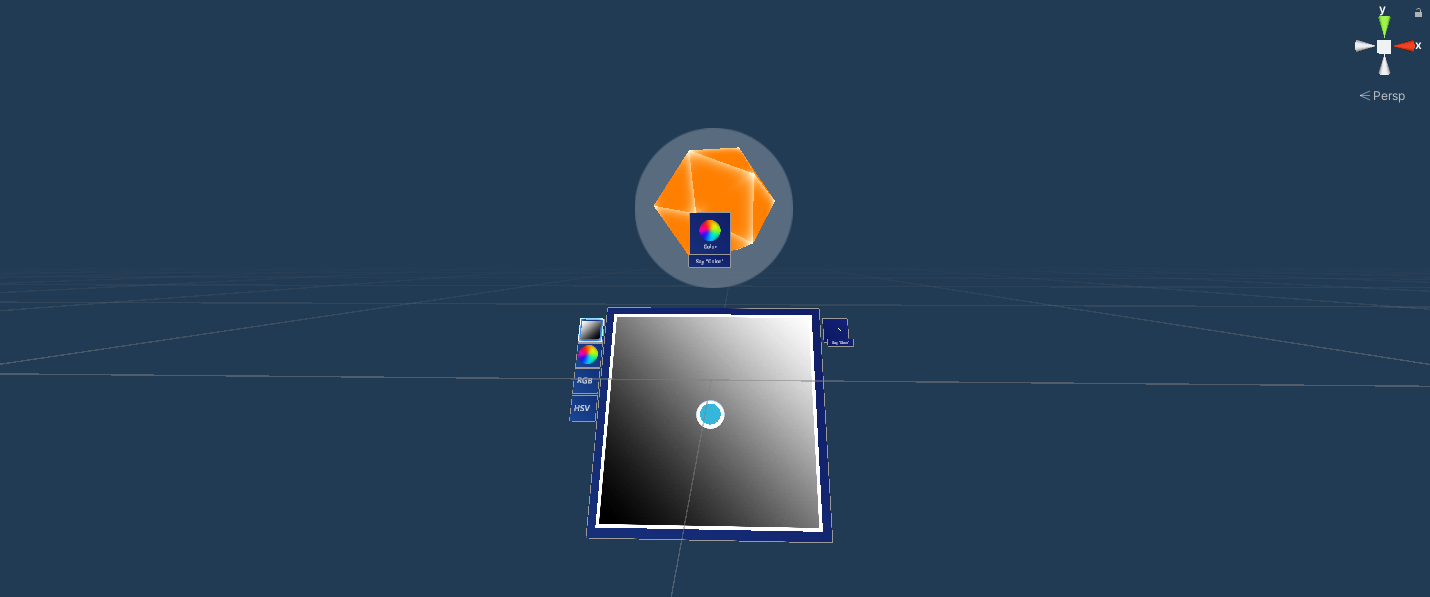
\includegraphics[width=0.9\linewidth]{figures/ColorPickerWidget.png}
  \caption{Color Picker Widget Game Object Prefab. Can select and visualize the Color Item in RGB and HSV formats.}
  \label{fig:ColorPickerWidget-figure}
\end{figure}

For new ways of interacting with IoT devices, tag-based Widgets can be added to an Item. Widgets such as Pressure sensor, Gesture sensor, Audio and Video streaming sensors, Sight sensor expand the possibilities of interaction with devices in virtual reality and are also used to simulate real-life interactive elements. At the moment, there are 12 tag-based Widgets in the NUIX-Studio Development kit. 

For different IoT scenarios, these tag-based Widgets can perform various functions. The platform provides three different environments: Smart Driving, Smart Classroom, and Smart Home environments. In the example scenario, the smartphone changes its mode based on the environment it is located in at the moment. Developers can create their own devices using the Thing Designer tool, and the platform will automatically understand in which environment the device is currently located and adjust its functionality to the given environment. 

\begin{figure}
  \centering
  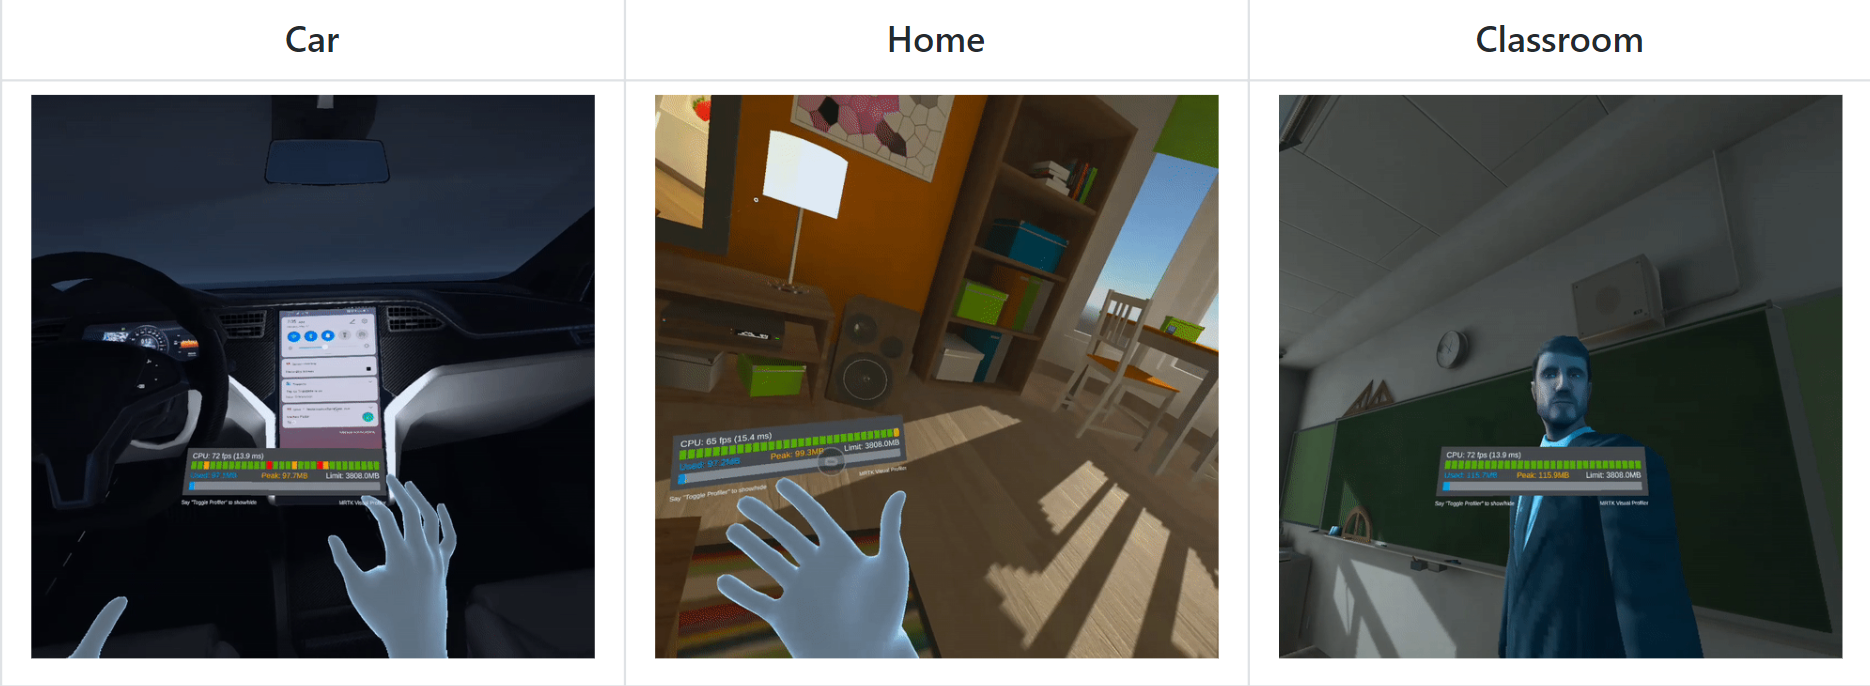
\includegraphics[width=0.9\linewidth]{figures/Environments.png}
  \caption{Three different environments that can be used by developers.}
  \label{fig:Environments-figure}
\end{figure}

\section{Complex computations API}

With the transfer of resource-intensive calculations to a separate server, it becomes possible to perform more reliable physical object simulations. Computations such as processing light, sound, and electromagnetic waves of other frequencies and various substances such as gas, water, are only limited by existing algorithms. 

Storing important physical parameters is sometimes critical for prototyping AIoT projects. For example, the next chapter shows how computing lighting on a separate instance can dramatically improve the user experience. Developers are provided with a tool for storing and synchronizing data for computing physics on the server. Thus, each of the instances can use the result of the computations while using the device's resources only for displaying them. 

\section{API and tools for IoT data visualization and analysis}

Each of IoT devices is visualized through Widgets, but designing Widgets by 3D modeling requires additional time. If a 3D model of the device already exists, the researcher can add it to the platform as a Widget and then connect extra Widgets to it. However, in the IoT environment used, not every device has a corresponding 3D model. There are several solutions to this problem. The first solution is to use 3D models of similar devices. Yet, it is not always possible to find the particular model, or sometimes the quality of these models does not meet the requirements. The second solution is device scanning. With the help of 3D scanners based on depth cameras, it is already possible to scan things with acceptable accuracy and at a relatively affordable price. If millimeter precision scanning is required, then expensive professional solutions can be used.

The resulting Widgets of 3D models can be added to Virtual reality. In the case of the NUIX-Studio App, scenes representing different environments are used. Scenes can be created within Unity editor and by using the Things designer,  or by interpreting the surrounding objects as Widgets (for example, people's position on the street is represented as an Item of Location type). This approach takes a long time to construct a scene, especially if one needs to use a copy of the real environment in Virtual reality. To reduce the time spent on 3D modeling, researchers can use solutions such as 3D scanning of the environment (Figure~\ref{fig:RoomScan-figure}). It is possible to scan the environment with good accuracy on many different smartphones using Depth Lab from Google (Figure~\ref{fig:Object_placement-figure}) and with excellent accuracy on the iPhone using Apple ARKit~\cite{baek_two-dimensional_2020, breitbarth_measurement_2019}. However, these scans of the environment are static scenes. If an object inside this environment is moved, then the scan will have to be performed again. Unfortunately, there is currently no solution to this problem. However, in the next chapter, it will be shown that the platform can be adapted to work with augmented reality, thus eliminating the need to match the real world with the virtual one fully.


\begin{figure}
  \centering
  \subcaptionbox{Depth Lab provides a functionality of placing virtual objects in real world. NUIX-Studio development kit provides API for exporting the Virtual Game Objects into Depth lab to visualize them in real world.\label{fig:Object_placement-figure}}
    {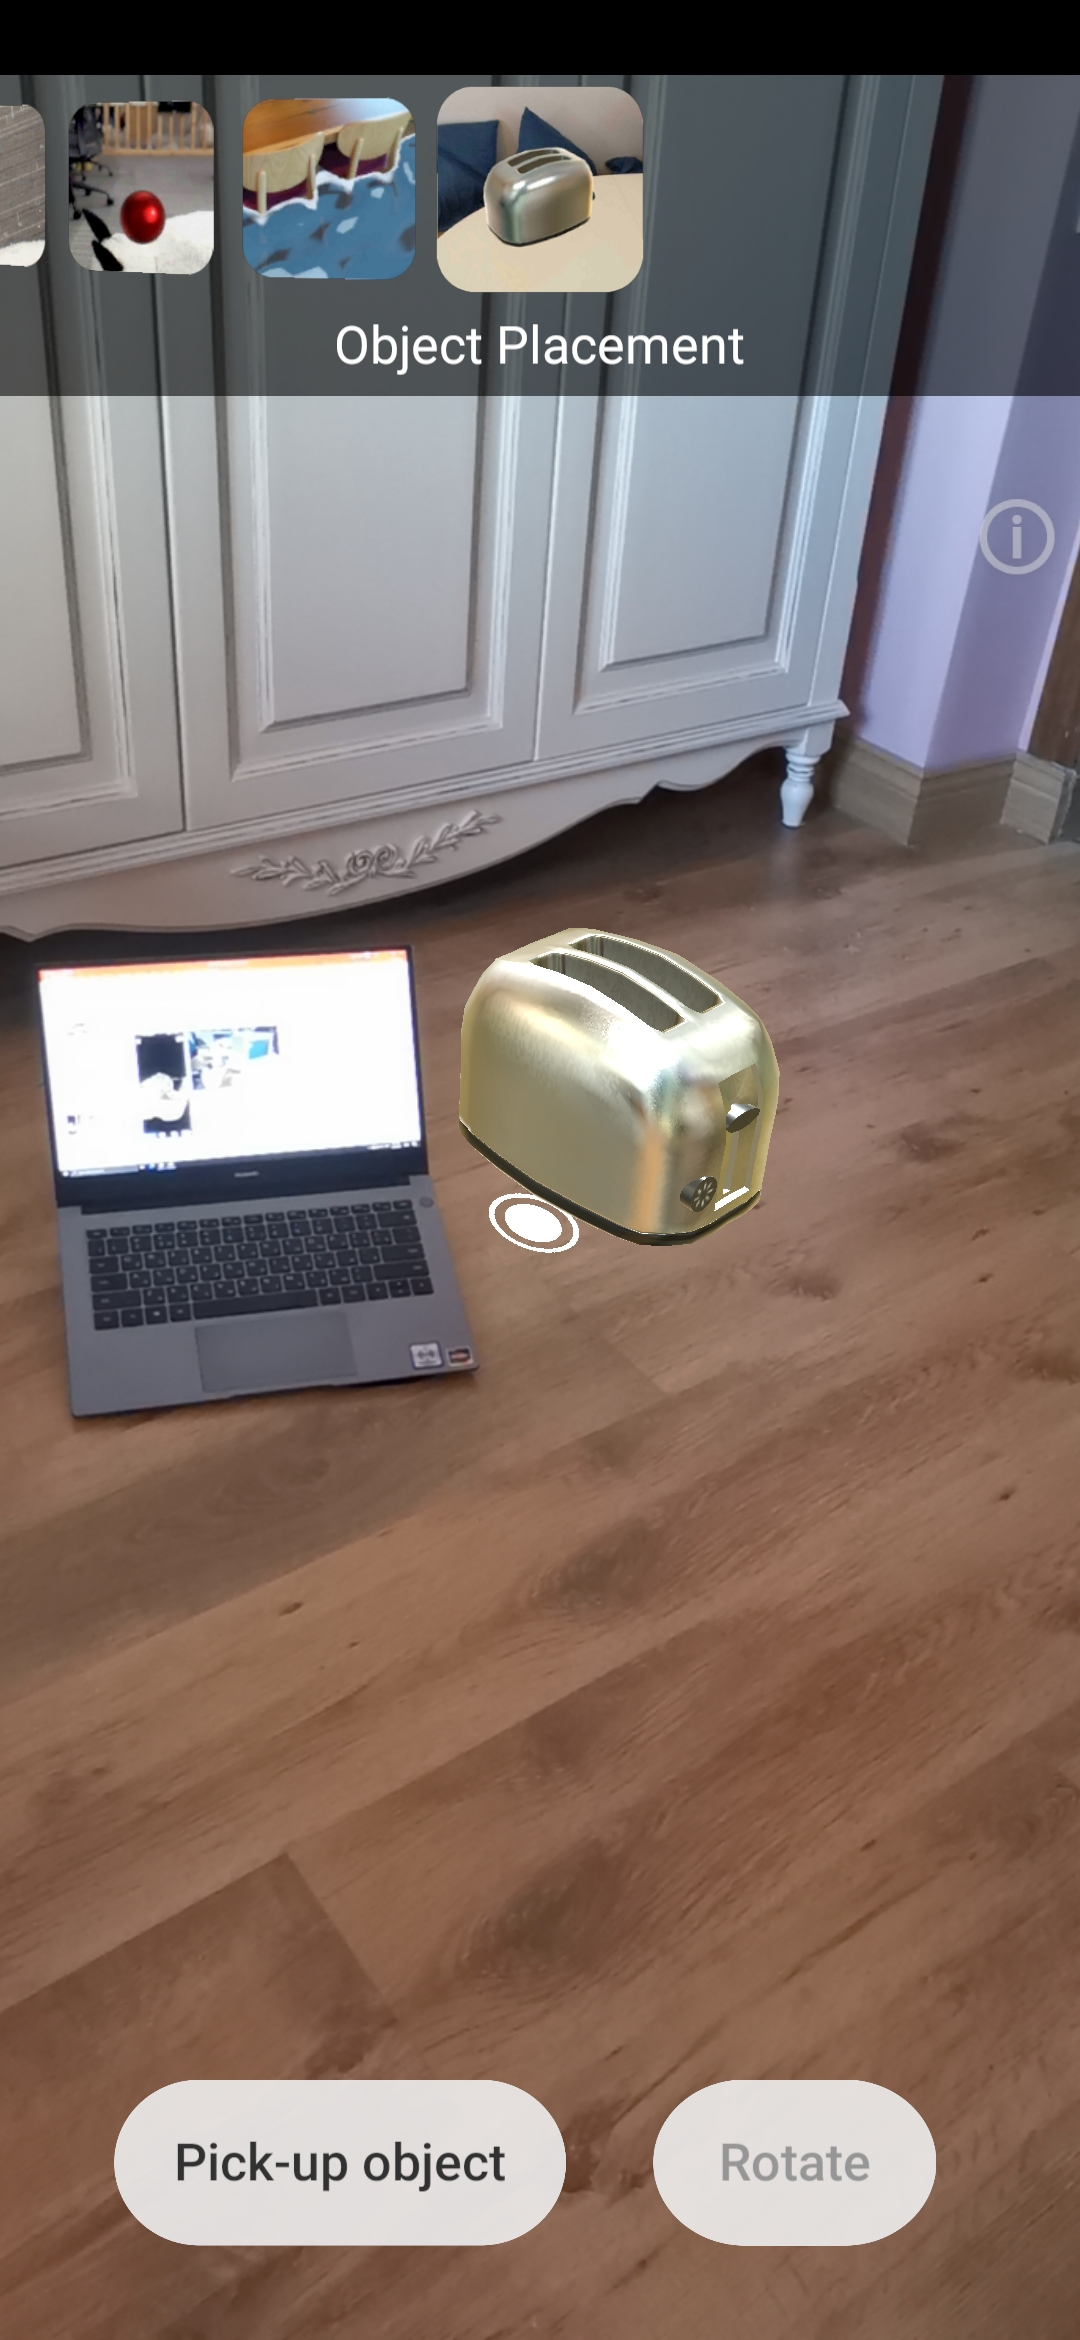
\includegraphics[width=0.45\linewidth]{figures/Object_placement.jpg}}
  \subcaptionbox{3D Scan of a room performed on the Huawei Phone. It can be seen that the scan quality is not ideal.\label{fig:RoomScan-figure}}
    {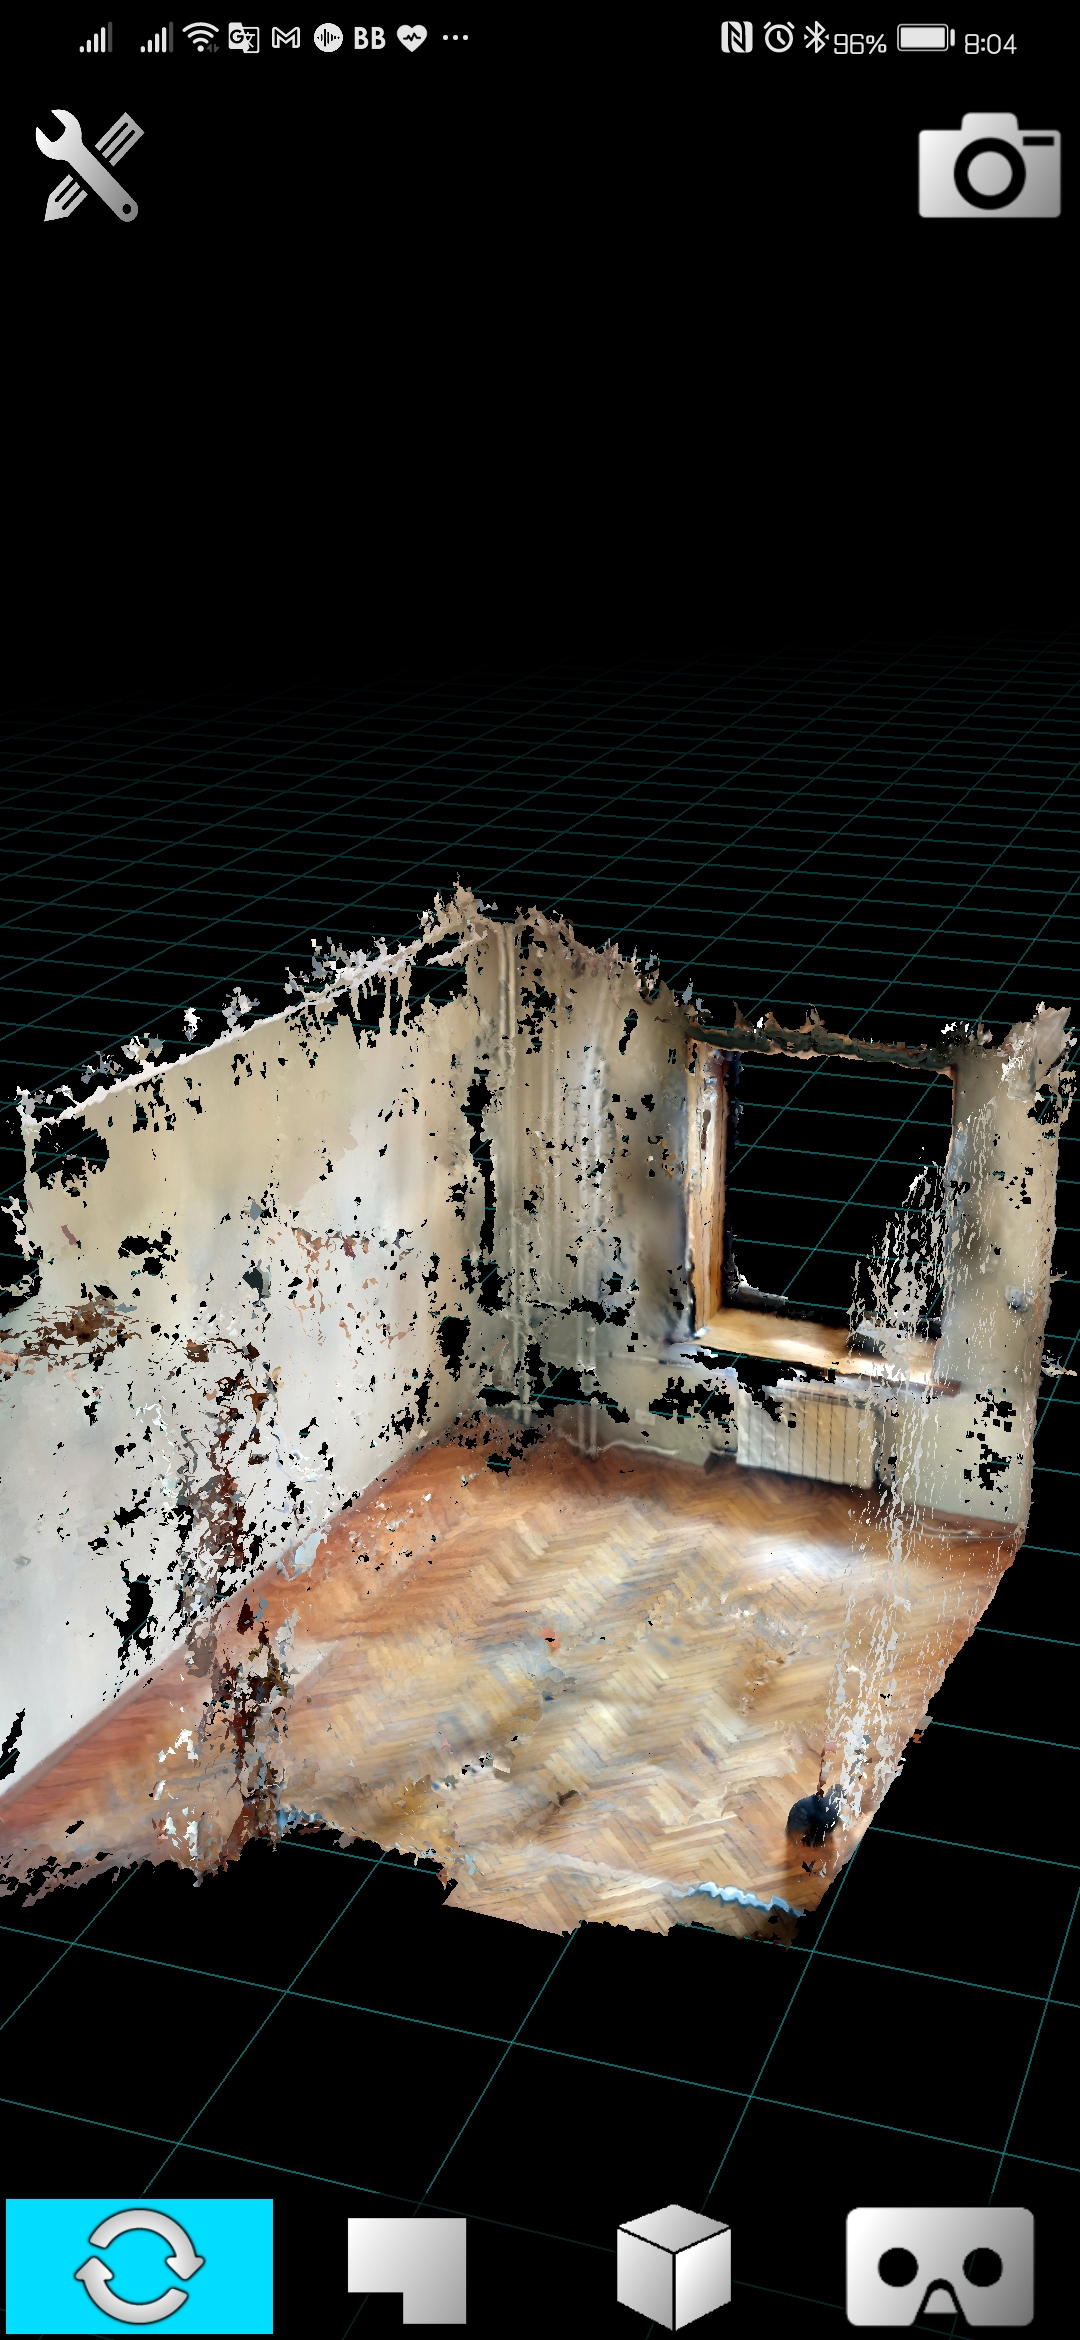
\includegraphics[width=0.45\linewidth]{figures/RoomScan.jpg}}
  \caption{Real world 3D scanning for extending it with virtual devices.}
  \label{fig:exp-screenshot}
\end{figure}

Various devices can track the movement of real IoT devices in the real world, such as Bluetooth tags, QR codes, magnetic field sensors, etc. Researchers can use the API to change the position of each Widget. Thus, when the device's position in the real world changes, the device's Widgets position in the virtual world will also change. It is also possible to perform the opposite action, but this requires a device that will move IoT devices in the real world.

Since changes in Items values are periodically written to the server, they can be visualized using the built-in system tools (Figure~\ref{fig:PersistenceExample-figure}) or further analyzed using external frameworks providing useful insights.

\begin{figure}
  \centering
  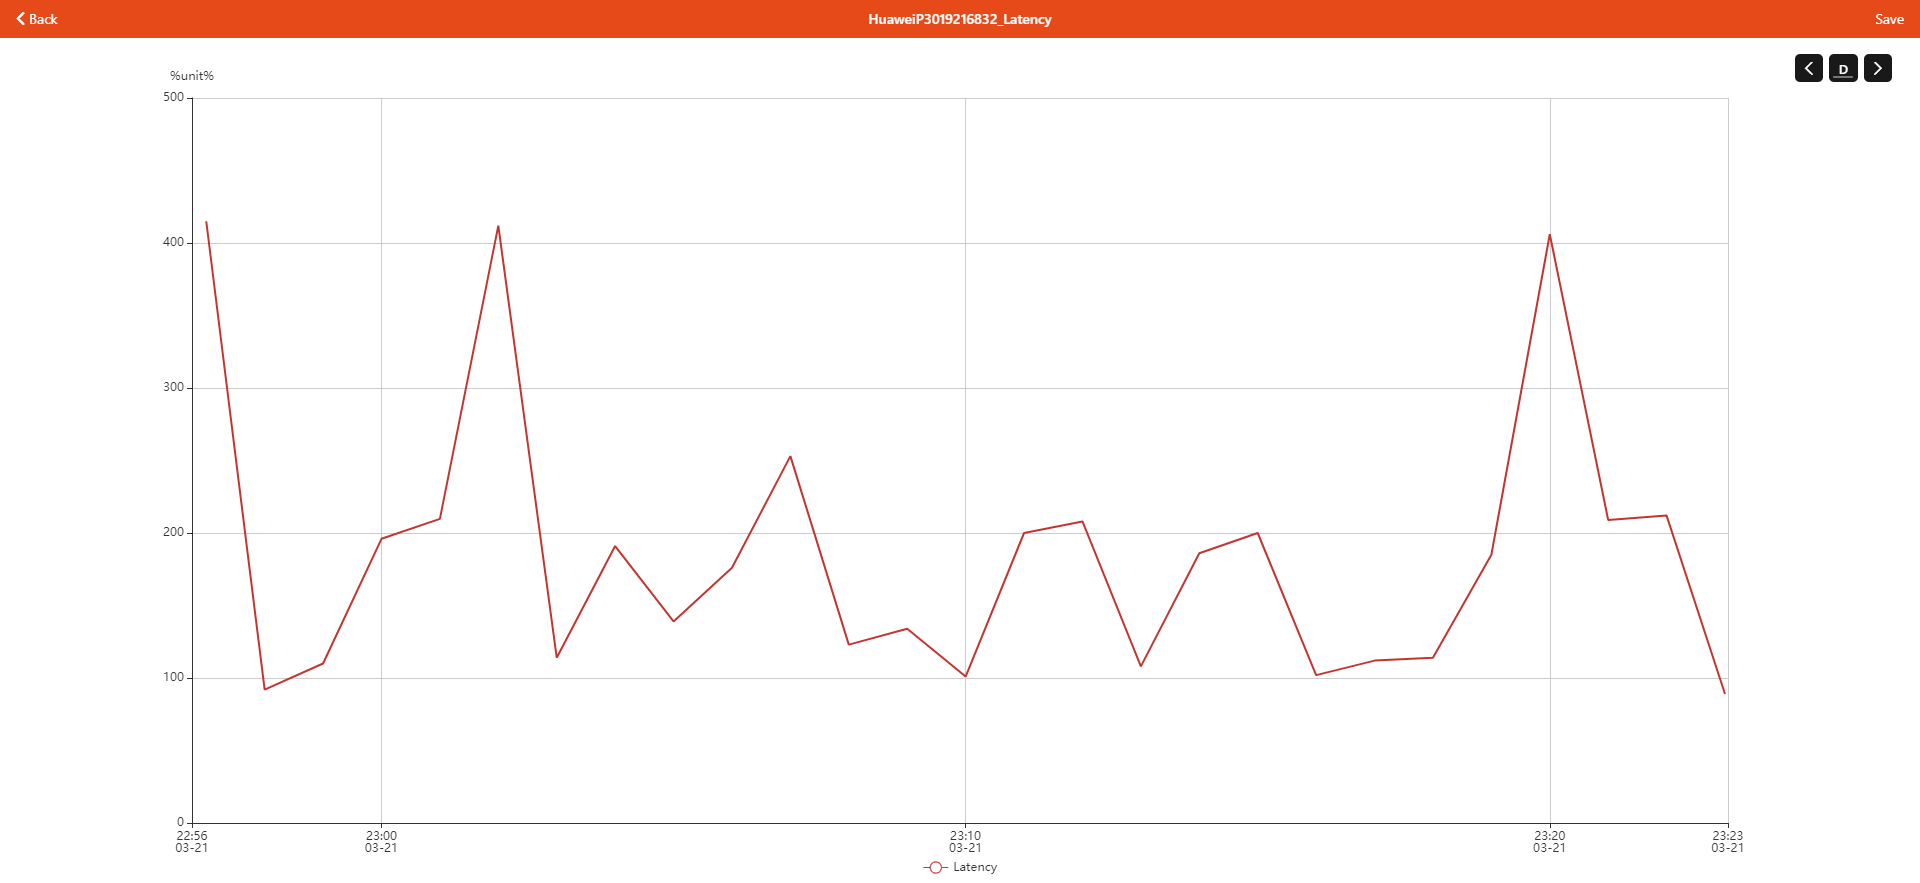
\includegraphics[width=0.9\linewidth]{figures/PersistenceExample.png}
  \caption{Persistence example: Latency value for accessing a remote device (in ms). }
  \label{fig:PersistenceExample-figure}
\end{figure}

\section{API for creating Widgets}

The platform provides only basic Widgets for the Items. These Widgets are used to give an example of how to visualize the IoT devices' data. By using this API, researchers can create Widgets specific to the device they develop. However, most of the Widgets to be developed can be divided into two categories: Sensor Widgets and Visual Widgets.

A virtual sensor Widget has been developed already. By using this Widget, researchers only need to build functions that will activate this sensor. Thus, the time spent on developing widgets is significantly reduced. In addition, the platform provides access to a large number of UX building blocks using the Mixed Reality Toolkit. Using this toolkit, the user will not need to spend time designing various buttons and switches. 


\begin{figure}
  \centering
  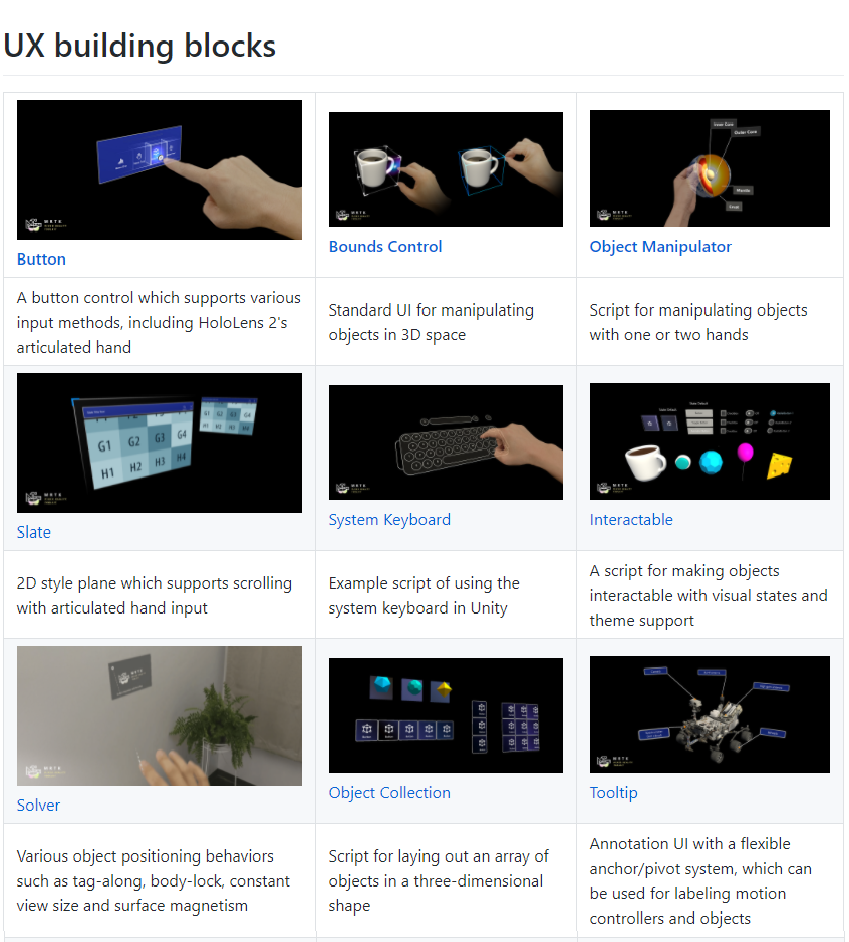
\includegraphics[width=0.6\linewidth]{figures/MRTK.png}
  \caption{UX building blocks.}
  \label{fig:MRTK-figure}
\end{figure}

\section{Summary}

With the help of the NUIX-Studio development kit, researchers can already create prototypes of projects for various AIoT scenarios. The toolkit provides a wide range of different widgets for developing new devices in virtual reality. In addition, the platform helps researchers to connect them with real-world devices in a relatively short time. Additionally, the platform allows developers to receive and send data to various AR applications. As a result, the developer can carry out an entire cycle of prototyping projects with a minimum investment of time and effort into development.